\documentclass[a4paper, 12pt]{article}

\usepackage[portuges]{babel}
\usepackage[utf8]{inputenc}
\usepackage{amsmath}
\usepackage{indentfirst}
\usepackage{graphicx}
\usepackage{float}
\usepackage{hyperref}
\usepackage{graphicx}
\usepackage{rotating}

\newcommand\tab[1][20pt]{\hspace*{#1}}

\begin{document}
%\maketitle

\begin{titlepage}
	\begin{center}
	
	\begin{figure}[!ht]
	\centering
	
\includegraphics[width=10cm]{unifesp.png}
	\end{figure}

		\Huge{Universidade Federal de São Paulo}\\
		\vspace{15pt}
        \vspace{95pt}
        \textbf{\LARGE{Laboratório de Sistemas Computacionais: Arquitetura e Organização de Computadores}}\\
		\vspace{2,5cm}
	\end{center}
	
	\begin{flushleft}
		\begin{tabbing}
			Professor Dr. Sérgio Ronaldo\\
			Leonardo Courbassier Martins\\
			103230
	\end{tabbing}
 \end{flushleft}
	%\vspace{1cm}
	
	\begin{center}
		\vspace{\fill}
			 Abril\\
		 2018
			\end{center}
\end{titlepage}
%%%%%%%%%%%%%%%%%%%%%%%%%%%%%%%%%%%%%%%%%%%%%%%%%%%%%%%%%%%
\tableofcontents

\newpage
% % % % % % % % % % % % % % % % % % % % % % % % % % %
\section{Introdução}
A arquitetura e a organização de um computador é fundamental e única em cada sistema que existe. A partir deles, é possível comparar diferentes processadores e sabendo a filosofia de cada um deles, é possível escolher um que mais se adequa a um determinado projeto.\\
É indiscutível que o processador é uma das partes mais importantes de um computador e, por isso, deve ser projetada com cautela e com técnicas cada vez mais aprimoradas para construir processadores cada vez mais rápidos e completos.\\
A mudança do tamanho de computadores é um bom exemplo de como uma boa organização do computador pode fazer diferença e que é necessário, cada vez mais, um desenvolvimentos de ténicas para uma tecnologia cada vez mais avançada.

\section{Objetivos}
O objetivo desse relatório é mostrar como é complexo a implementação de um processador simples, e que é necessário várias técnicas e considerações antes de seu \textit{design} para determinar qual é o objetivo do processador e para que ele está sendo desenvolvido.\\
Foi utilizado o Quartus II (\cite{quartus}) para a implementação do processador e testes.
\newpage

\section{Fundamentação Teórica}
\subsection{Processador}
O processador é uma parte de um sistema computacional, que utiliza de um conjunto de instruções para executar a aritmética básica, lógica, e a entrada e saída de dados. O processador tem um papel parecido ao cérebro no computador, pois ele controla todo os periféricos do computador e é o núcleo dele.\\
Além de saber o para quê serve, uma pergunta mais interessante é: Como funciona um processador?\\
Como é feita a implementação de um processador? Além dessas perguntas, é necessário conhecer o público-alvo do processador. O processador será projetado para programadores (dando várias instruções diferentes e diversas opções) ou será projetado para usuários comuns?
A resposta para essas perguntas dividem o processador em várias técnicas de \textit{design}.\\
As suas implementações vem mudando drásticamente desde o primeiro processador (Intel 4004, em 1971), assim como a tecnologia também vem desenvolvendo-se, surgiram diversas arquiteturas, organizações, entre outros. Já foram testados várias combinações de organizações até a que compreende-se como a melhor atualmente.

\subsection{Arquitetura}
Dentre os diversos tipos de arquitetura existentes, as mais conhecidas são as arquiteturas RISC (\textit{Reduced Instruction Set Computer}) e CISC (\textit{Complex Instruction Set Computer}).\\
A estratégia de \textit{design} RISC foca-se em um número pequeno de instruções, diminuindo o CPI (\textit{Clock per Instruction}) e a complexidade do processador.\\
Em contrapartida, a estratégia CISC foca-se em um número grande de instruções, o que facilita muito a programação, com várias instruções complexas, e com isso, a complexidade dos programas feitos em máquinas CISC são menores (em relação ao número de instruções).
Geralmente, as instruções tem um maior CPI, mas isso é compensado com uma funcionalidade não trivial.
Foi escolhido o modelo de arquitetura RISC para este relatório.\\

\subsection{MIPS}
Como referência de processador, foi utilizado o MIPS. O MIPS é um estilo de processador que não tem um único processador físico. 
\\
Quando foi comercializado em 1981, era comercializado a ideia do processador e outras empresas faziam a implementação delas. Sua característica principal é ser muito simples e didático e ele foi um grande influenciador das próximas arquiteturas RISC.\\
A sua implementação com \textit{pipeline} é bem rápida e não é tão complexa, e seus programas não ficam muito complexos.\\
O MIPS contém 32 registradores em sua implementação e alguns deles são reservados para o sistema. Além disso ele possui uma unidade de controle que facilita todo o controle do processador e seus componentes.\\

\newpage
\section{Desenvolvimento}
Essa seção mostra os pontos principais da implementação do processador. O processador aqui aprensetado é monociclo, sem \textit{pipeline} e RISC. Contém 28 instruções (discutidas nas próximas seções) e 5 tipos de formatos de instruções.\\
Além disso, ele possui 32 registradores de 32 bits, mas apenas alguns de próposito geral.

\subsection{Formato das Instruções}
Antes da implementação do processador, é necessário definir os formatos de instruções que será utilizado. A tabela abaixo contém todos os 5 formatos, divindo os bits e os campos de cada formato.
\begin{center}
\begin{tabular}{ cl }
 	\textbf{Tipo} & \textbf{Campos}\\
 	1 & [ OpCode / RegDest / RegOrigem / RegAlvo /\ | ]\\
 	  &  \ \ [31:27]\ \ \ \ \ \ [26:22]\ \ \ \ \ \ \ \ [21:17]\ \ \ \ \ \ \ \ [16:12]\ \ \ [11:0]\\
 	\hline
 	\\
 	2 & [ OpCode / RegDest / RegOrigem / Imediato (ou |) ]\\
 	  &  \ \ [31:27]\ \ \ \ \ \ [26:22]\ \ \ \ \ \ \ \ [21:17]\ \ \ \ \ \ \ \ \ \ \ [16:0]\\
 	\hline
 	\\
 	3 & [ OpCode / RegDest / RegOrigem (ou |) / Imediato (ou |) ]\\
 	  &  \ \ [31:27]\ \ \ \ \ \ [26:22]\ \ \ \ \ \ \ \ \ \ \ [21:17]\ \ \ \ \ \ \ \ \ \ \ \ \ \ \ \ \ \ \ \ [16:0]\\
 	\hline
 	\\
 	4 & [ OpCode / RegDest / Imediato ]\\
 	  &  \ \ [31:27]\ \ \ \ \ \ [26:22]\ \ \ \ \ \ \ \ [21:0]\\
 	\hline
 	\\
 	5 & [ OpCode /\ | ]\\
 	  &  \ \ [31:27]\ \ \  [26:0]\\
 	\hline
  \end{tabular}
 \end{center}
  
O tipo 1 destina-se a operações aritméticas com 3 registradores e sem imediato. Já o tipo 2, destina-se a operações aritméticas com 2 registradores e um imediato. O tipo 3, destina-se aos desvios de fluxos condicionais e incondicionais. O tipo 4, destina-se as instruções de entrada e saída, comunicação que será desenvolvida mais adiante. Já o tipo 5, destina-se as instruções de controle do processador.

\subsection{Conjunto de Instruções}
A tabela abaixo contém todo o conjunto de instruções que o processador terá, os tipos das instruções e seu opCode.
\begin{center}
\begin{tabular}{ ccc }
 	\textbf{OpCode} & \textbf{Instrução} & \textbf{Tipo}\\
 	00000 & Add & 1\\
 	00001 & Addi & 2\\
 	00010 & Sub  & 1\\
 	00011 & Subi & 2\\
 	00100 & Mult & 1\\
 	00101 & Multi & 2\\
 	00110 & Div & 1\\
 	00111 & Divi & 2\\
 	01000 & Mod & 1\\
 	01001 & Slt & 1\\	
 	01010 & Slti & 2\\
 	01011 & And & 1\\
 	01100 & Andi & 2\\
 	01101 & Or & 1\\
 	01110 & Ori & 2\\
 	01111 & Not & 2\\
 	10000 & ShR & 2\\
 	10001 & ShL & 2\\
 	10010 & Load & 4\\
 	10011 & Loadi & 4\\
 	10100 & Store & 4\\
 	10101 & Jump & 3\\
 	10110 & Beq & 3\\
 	10111 & Bne & 3\\
 	11000 & Nop & 5\\
 	11001 & Halt & 5\\
 	11010 & In & 4\\
 	11011 & Out & 4\\
 	11100 & Mov & 2\\
  \end{tabular}
\end{center}

\subsection{Registradores}
Como no MIPS, o processador também utilizará de 32 registradores e alguns deles serão limitados ao processador. A tabela abaixo descreve todos os registradores e suas funções.
\begin{center}
\begin{tabular}{ ccc }
 	\textbf{Nome} & \textbf{Número} & \textbf{Descrição}\\
 	\$0 & 00 & \$zero: Constante zero\\
 	\$1 & 01 & \$at: Reservado\\
 	\$2 & 02 & \$v0: Resultado de uma função\\
 	\$3 & 03 & \$v1: Resultado de uma função\\
 	\$4 & 04 & \$a0: Argumento para uma função\\
 	\$5 & 05 & \$a1: Argumento para uma função\\
 	\$6 & 06 & \$a2: Argumento para uma função\\
 	\$7 & 07 & \$a3: Argumento para uma função\\
 	\$8 & 08 & \$t0: Uso geral\\
 	\$9 & 09 & \$t1: Uso geral\\
 	\$10 & 0A & \$t2: Uso geral\\
 	\$11 & 0B & \$t3: Uso geral\\
 	\$12 & 0C & \$t4: Uso geral\\
 	\$13 & 0D & \$t5: Uso geral\\
 	\$14 & 0E & \$t6: Uso geral\\
 	\$15 & 0F & \$t7: Uso geral\\
 	\$16 & 10 & \$s0: Uso geral (salvo em chamadas de função)\\
 	\$17 & 11 & \$s1: Uso geral (salvo em chamadas de função)\\
 	\$18 & 12 & \$s2: Uso geral (salvo em chamadas de função)\\
 	\$19 & 13 & \$s3: Uso geral (salvo em chamadas de função)\\
 	\$20 & 14 & \$s4: Uso geral (salvo em chamadas de função)\\
 	\$21 & 15 & \$s5: Uso geral (salvo em chamadas de função)\\
 	\$22 & 16 & \$s6: Uso geral (salvo em chamadas de função)\\
 	\$23 & 17 & \$s7: Uso geral (salvo em chamadas de função)\\
 	\$24 & 18 & \$t8: Uso geral\\
 	\$25 & 19 & \$t9: Uso geral\\
 	\$26 & 1A & \$k0: Reservado\\
 	\$27 & 1B & \$k1: Reservado\\
 	\$28 & 1C & \$gp: Ponteiro global\\
 	\$29 & 1D & \$sp: Ponteiro da pilha\\
 	\$30 & 1E & \$fp: Ponteiro do frame\\
 	\$31 & 1F & \$ra: Endereço de retorno\\
  \end{tabular}
\end{center}
A mentalidade por trás dessa divisão de registradores está na usabilidade em programas mais complexos com chamadas recursivas e várias funções. Além de uma possível pilha para outros objetivos além da recursão.

\subsection{Esquemático}
\begin{sidewaysfigure}[htp]
	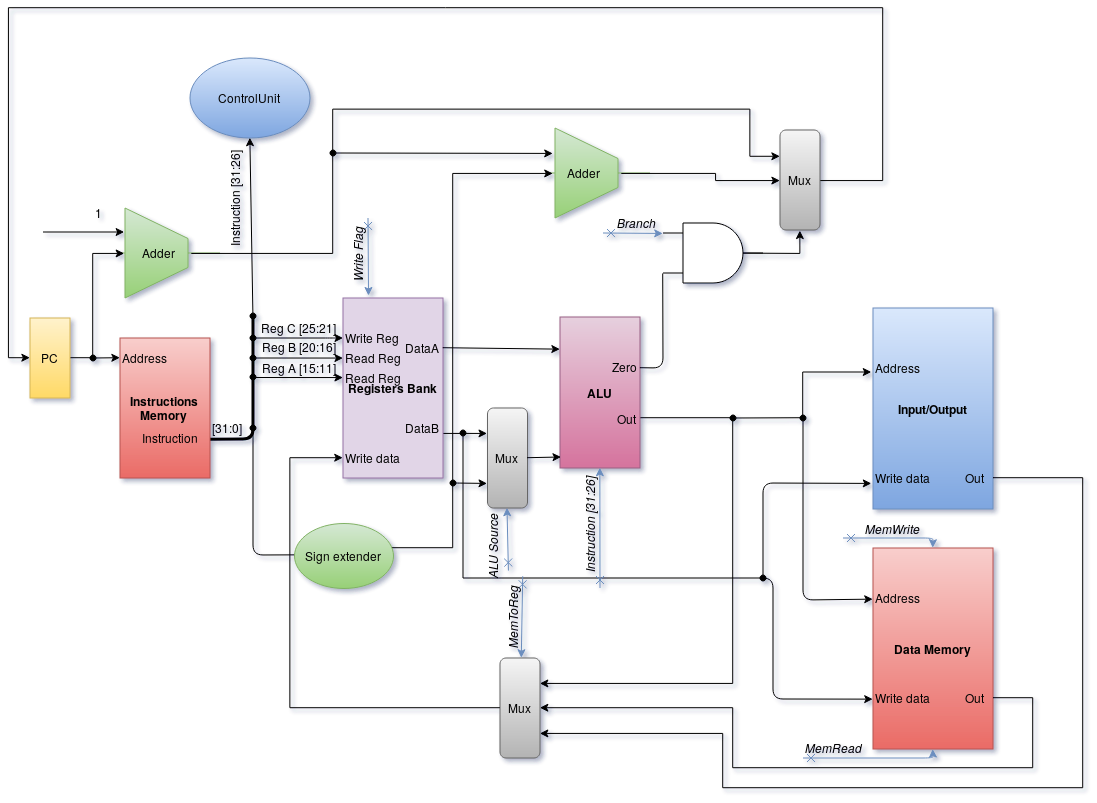
\includegraphics[scale=0.5]{LABAOC.png}
	\caption{Esquemático do processador}
\end{sidewaysfigure}
\newpage

\section{Conclusão}
A construção de um processador é um processo muito complexo devido as várias considerações de \textit{design} que são necessárias. A maior das escolhas é entre seguir a arquitetura RISC ou CISC, ambas tem pontos positivos muito interessantes (como discutido nas primeiras seções) e que facilitam em algum momento da construção do processador. Seja no começo com a implementação física dele (no caso do RISC) ou depois, na utilização do processador (no caso do CISC).\\
O resultado gerado atendeu as expectativas e objetivo do relatório, mostrando como é importante o estudo de arquitetura e organização de computadores.

\section{Trabalhos futuros}
Futuramente, será implementado o multiciclo ao processador e a comunicação através do GPIO do sistema embarcado arduino(\cite{arduino}).

\begin{thebibliography}{9}

\bibitem{quartus}
  \textit{Software} Quartus:\\
  \url{https://www.altera.com/products/design-software/fpga-design/quartus-prime/overview.html}

\end{thebibliography}

\end{document}



